%{{{ Preamble

\documentclass{article}
\usepackage{graphicx}
\graphicspath{{./}{../FIGs/}{../Logos/}}
\ifx\HCode\Undef
\DeclareGraphicsExtensions{.pdf,.png}
\else
\usepackage{tex4ht}
\DeclareGraphicsExtensions{.svg, .png, .jpg}
\fi
\usepackage{hyperref}
\usepackage{color}

%\renewcommand{\rmdefault}{ptm}
%\renewcommand\familydefault{\sfdefault}

%}}}

%{{{ Front

\newcommand{\luxunda}{%
\begin{tabular}{c}
  Crist\'obal Medina L\'opez, \\
  Juan Pablo Garc\'ia Ortiz and \\
  Juan Alvaro Mu\~noz Naranjo. \\
  ~\\
  \href{http://www.luxunda.es/}{Luxunda SA}
\end{tabular}
}

\newcommand{\SAL}{%
\begin{tabular}{c}
  Leocadio Gonz\'alez Casado and \\
  Vicente Gonz\'alez Ruiz.\\
  ~\\
  \href{http://www.hpca.ual.es/}{SAL, UAL}
\end{tabular}
}

\author{%
Crist\'obal Medina L\'opez, Juan Pablo Garc\'ia Ortiz and Juan Alvaro Mu\~noz Naranjo,\\\href{http://www.luxunda.es/}{Luxunda SL}. \\
~\\
Leocadio Gonz\'alez Casado and Vicente Gonz\'alez Ruiz,\\\href{http://www.hpca.ual.es/}{SAL, UAL}.
}

%\begin{tabular}{cc}%
%  \luxunda &  \SAL %
%\end{tabular}%

\newcommand{\thankss}{
%{{{
  
  \vbox{
    \ifx \HCode\Undfef
    \else
    \HCode{<div style="text-align:center;">
      <img width=800 src="http://slides.p2psp.org/2014-11-Jornada-Contenidos-Digitales-UAL/FIGs/thanks.svg" align="top"/>
      </div>
    }
    \fi
  }
  
%}}}
}  

%\title{IP-TV over P2PSP Teams}
\title{Live-Video Streaming over Internet using P2PSP}
\date{Jan 21, 2015 \\~\\ \url{http://slides.p2psp.org/2015-01-Elche} \\~\\ \thankss}

%}}}

\begin{document}
%{{{ Body

%{{{ Font

% Family       Font Name
% pag          Avant Garde *
% fvs          Bitstream Vera Sans
% pbk          Bookman
% bch          Charter
% ccr          Computer Concrete
% cmr          Computer Modern
% pcr          Courier
% mdugm        Garamond
% phv          Helvetica *
% fi4          Inconsolata
% lmr          Latin Modern
% LinuxBiolinumT-OsF     Linux Biolinum (formerly 'fxb' in older package versions)
% LinuxLibertineT-OsF    Linux Libertine (formerly 'fxl' in older package versions)
% pnc          New Century Schoolbook
% ppl          Palatino
% ptm          Times
% uncl         Uncial
% put          Utopia
% pzc          Zapf Chancery

%\fontfamily{pag}\selectfont
\fontfamily{phv}\selectfont
%\sffamily
%\def\normalfont{\sffamily}
%\renewcommand{\familydefault}{cmss} \
%\renewcommand{\familydefault}{\sfdefault}
%\selectfont

%}}}

\maketitle


\section{Digital Video Broadcasting (DVB)}
%{{{

\ifx \HCode\Undfef
%\begin{center}
%  \includegraphics[width=1.0\textwidth]{DVB}
%\end{center}
\else
\HCode{
  <div style="text-align:center;">
    <img height="600" src="http://slides.p2psp.org/2014-11-Jornada-Contenidos-Digitales-UAL/FIGs/DVB.svg" />
  </div>
}
\fi

%}}}

\section{Internet Protocol (IP)}
%{{{

\ifx \HCode\Undfef
%\begin{center}
%  \includegraphics[width=1.0\textwidth]{world-internet}
%\end{center}
\else
\HCode{
  <div style="text-align:center;">
    <img height="500" src="http://slides.p2psp.org/2014-11-Jornada-Contenidos-Digitales-UAL/FIGs/world-internet.svg" />
  </div>
}
\fi

%}}}

\section{Video on Demand over the Internet (IP-VoD)}
%{{{

\ifx \HCode\Undfef
%\begin{center}
%  \includegraphics[width=1.0\textwidth]{http://slides.p2psp.org/2014-11-Jornada-Contenidos-Digitales-UAL/FIGs/spain-IPVoD}
%\end{center}
\else
\HCode{
  <div style="text-align:center;">
    <img height="600" src="http://slides.p2psp.org/2014-11-Jornada-Contenidos-Digitales-UAL/FIGs/spain-IPVoD.svg" />
  </div>
}
\fi

%}}}

\section{Television over the Internet (IP-TV)}
%{{{

\ifx \HCode\Undfef
%\begin{center}
%  \includegraphics[width=1.0\textwidth]{http://slides.p2psp.org/2014-11-Jornada-Contenidos-Digitales-UAL/FIGs/spain-IPTV-Hub}
%\end{center}
\else
\HCode{
  <div style="text-align:center;">
    <img height="600" src="http://slides.p2psp.org/2014-11-Jornada-Contenidos-Digitales-UAL/FIGs/spain-IPTV-Hub.svg" />
  </div>
}
\fi

%}}}

\section{IP-TV over IP Unicast}
%{{{

\ifx \HCode\Undfef
%\begin{center}
%  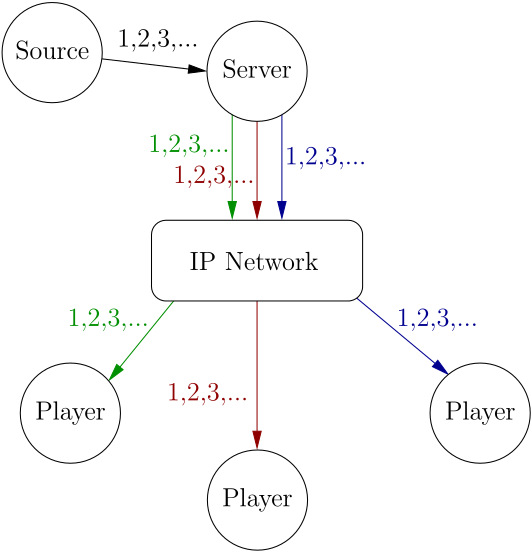
\includegraphics[width=1.0\textwidth]{unicast-server}
%\end{center}
\else
\HCode{
  <div style="text-align:center;">
    <img height="600" src="http://slides.p2psp.org/2014-11-Jornada-Contenidos-Digitales-UAL/FIGs/unicast-server.svg" />
  </div>
}
\fi
% <object
%   height="750" data="unicast-hub.svg" type="image/svg+xml" align="middle" 
% </object>
% }

%}}}

\section{IP-TV over IP Multicast (also P2PSP using IP Multicast)}
%{{{

\ifx \HCode\Undfef
%\begin{center}
%  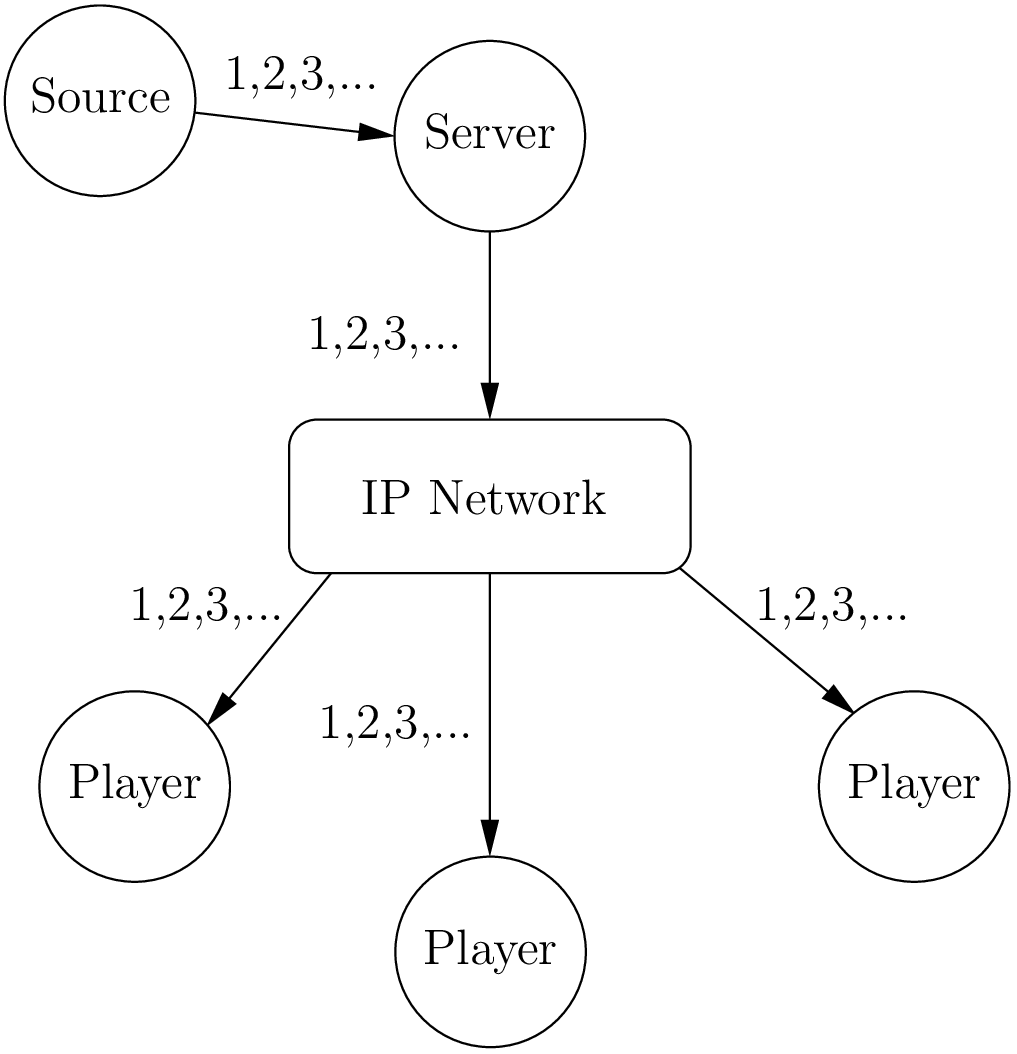
\includegraphics[width=1.0\textwidth]{multicast-server}
%\end{center}
\else
\HCode{
  <div style="text-align:center;">
    <img height="600" src="http://slides.p2psp.org/2014-11-Jornada-Contenidos-Digitales-UAL/FIGs/multicast-server.svg" />
  </div>
}
\fi

%}}}

\section{IP-TV over P2PSP (using IP Unicast)}
%{{{

\ifx \HCode\Undfef
%\begin{center}
%  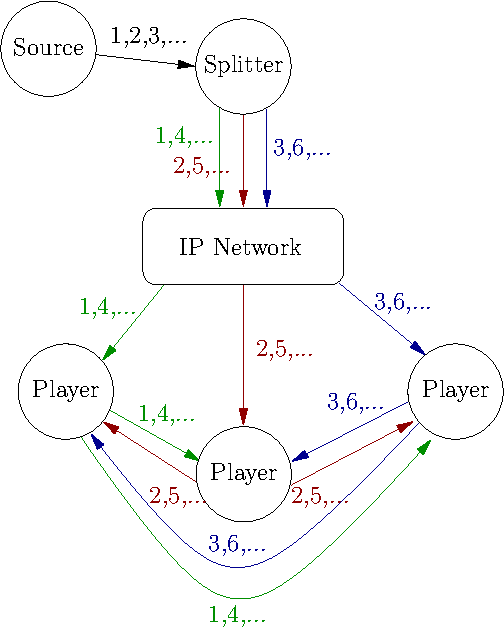
\includegraphics[width=1.0\textwidth]{unicast-splitter}
%\end{center}
\else
\HCode{
  <div style="text-align:center;">
    <img height="500" src="http://slides.p2psp.org/2014-11-Jornada-Contenidos-Digitales-UAL/FIGs/unicast-splitter.svg" />
  </div>
}
\fi

\begin{itemize}
\item The number of chunks sent peer peer does not depend on the team
  size.
\item The number of chunks that the splitter sends does not depend on
  the team size.
\end{itemize}

%}}}

\section{IP-TV over IP Unicast + P2PSP (revisited)}
%{{{

\ifx \HCode\Undfef
%\begin{center}
%  \includegraphics[width=1.0\textwidth]{spain-IPTV-P2P}
%\end{center}
\else
\HCode{
  <div style="text-align:center;">
    <img height="600" src="http://slides.p2psp.org/2014-11-Jornada-Contenidos-Digitales-UAL/FIGs/spain-IPTV-P2P.svg" />
  </div>
}
\fi

%}}}

\section{Where \& What is P2PSP}
%{{{

\begin{itemize}

\item \href{http://www.p2psp.org/en/}{P2PSP (Peer-to-Peer ``Straightforward'' Protocol)} is an open
  (\href{http://www.oxforddictionaries.com/definition/english/non-proprietary}{non-propietary})
  application-layer protocol for the real-time streaming of media
  content between networked entities.
\item An open-source (\href{https://www.gnu.org/copyleft/gpl.html}{GNU
    GPL v3}) implementation is available at
  \href{https://launchpad.net/p2psp}{here}.
\end{itemize}

% \section{P2PSP architecture vs. C/S architecture.}
% \begin{center}
%   \includegraphics[width=0.9\textwidth]{P2PSP_vs_CS}
% \end{center}
% Notice that:
% \begin{enumerate}
% \item The P2PSP's Splitter node (S in red) only sends a copy of the
%   stream regardless of the number of Peers (P). In a C/S system, the
%   Server (S in green) sends as many copies as Clients (C).
% \item If a link or a Peer fails in a P2PSP team, the lost chunks are
%   dispersed in time. Therefore, signal interpolation could be
%   efficiently used to hide to the users this lost of information.
% \end{enumerate}

%\large

%}}}
\section{P2PSP's Sets of Rules}
%{{{

\subsection{IP Mulicast Set (IMS) of rules}
%{{{

\begin{itemize}
\item The splitter sends chunks to peers using an IP multicast
  channel (notice that peers do not need to communicate each other).
\item Obviously, IP multicast must be avaiable!
\item The splitter runs using the {\tt --mcast} flag.
\item This Set is incompatible (does not make sense to use) with DBS,
  FNS, ACS, LRS, EMS, NTS and CIS.
\end{itemize}

\ifx \HCode\Undfef
%\begin{center}
%  \includegraphics[width=0.5\textwidth]{multicast-splitter}
%\end{center}
\else
\HCode{
  <div style="text-align:center;">
    <img height="600" src="http://slides.p2psp.org/2014-11-Jornada-Contenidos-Digitales-UAL/FIGs/multicast-splitter.svg" />
  </div>
}
\fi

%}}}

\subsection{Data Broadcasting Set (DBS) of rules}
%{{{

\ifx \HCode\Undfef
%\begin{center}
%  \includegraphics[width=0.5\textwidth]{congestion_control2}
%\end{center}
\else
\HCode{
  <div style="text-align:center;">
    <img height="500" src="FIGs/congestion_control2.svg" />
  </div>
}
\fi

\begin{itemize}
\item The splitter uses a Round-Robing broadcasting strategy and Unicast.
\item A peer sends the previusly received splitter's chunk to the next
  peer of their list of peers only when it receives a chunk from
  another peer.
\item All peers contribute equally (send the same amount of data).
\item Monitor(s) peer(s) report(s) lost chunks to the splitter.
\item The peers that are already in the team insert in their list of
  peers to those incomming peers that send a [Hello] or a chunk of
  data.
\item Peers maintain a unsupportivity counter for each other peer in
  the team that counts the difference between the number of chunks
  send to and the number of chunks received from that peer. These
  counters are divides by two periodically.
\item DBS is the default mode and incompatible with IMS.
\item The buffer size must be at last as large as the number of peers
  of the team.
\end{itemize}

%}}}

\subsection{Full-cone Nat Set (FNS) of rules}
%{{{

\begin{itemize}
\item Extends DBS.
\item Enables inbound UDP traffic between the splitter and the peer.
\item To achieve this, FNS-peers send a [Hello] (UDP) message to the
  splitter (using only DBS, peers send [Hello] messages to the rest of
  peers of the team when they arrive, but not to the splitter).
\end{itemize}

\ifx \HCode\Undfef
%\begin{center}
%  \includegraphics[width=0.5\textwidth]{IMS_DBS_FNS_timeline}
%\end{center}
\else
\HCode{
  <div style="text-align:center;">
    <img height="400" src="FIGs/IMS_DBS_FNS_timeline.svg" />
  </div>
}
\fi

%}}}

\subsection{Adaptive Chunk-rate Set (ACS)}
%{{{

\begin{itemize}
\item Extends DBS.
\item Peers can send a different amount of data, depending on their
  estimated capacity.
\item For every peer, the splitter gathers statistics from the
  monitor(s) peer(s) about the lost chunk ratio and estimates a
  capacity.
\item The unsupportivity counters threshold must be tuned carefully
  (they control when a peer decides to remove from his list of peer to
  other peer -- $P_1$ could remove $P_3$ --).
\end{itemize}

\ifx \HCode\Undfef
%\begin{center}
%  \includegraphics[width=0.5\textwidth]{ACS}
%\end{center}
\else
\HCode{
  <div style="text-align:center;">
    <img height="200" src="http://slides.p2psp.org/2014-11-Jornada-Contenidos-Digitales-UAL/FIGs/ACS.svg" />
  </div>
}
\fi

%}}}

\subsection{Lost chunks Recovery Set (LRS)}
%{{{

\begin{itemize}
\item Extends DBS.
\item Retransmit massively lost chunks (those that have not arrived to
  any monitor peer).
\item Lost chunks are transmitted by at leas one monitor peer.
\end{itemize}

\ifx \HCode\Undfef
%\begin{center}
%  \includegraphics[width=0.5\textwidth]{LRS}
%\end{center}
\else
\HCode{
  <div style="text-align:center;">
    <img height="200" src="http://slides.p2psp.org/2014-11-Jornada-Contenidos-Digitales-UAL/FIGs/LRS.svg" />
  </div>
}
\fi

%}}}

\subsection*{NAT: Network Address Translation}
%{{{

\ifx \HCode\Undfef
%\begin{center}
%  \includegraphics[width=0.5\textwidth]{NATting}
%\end{center}
\else
\HCode{
  <div style="text-align:center;">
    <img height="300" src="FIGs/NATting.svg" />
  </div>
}
\fi

%\subsection*{Static and dynamic NAT translaction}

%}}}

\subsection*{\href{http://en.wikipedia.org/wiki/Network_address_translation}{Cone NATs versus Symmetric NATs}}
%{{{

\ifx \HCode\Undfef
%\begin{center}
%  \includegraphics[width=0.5\textwidth]{cone-NAT}
%  \includegraphics[width=0.5\textwidth]{symmetric-NAT}
%\end{center}
\else
\HCode{
  <div style="text-align:center;">
    <img height="300" src="FIGs/cone-NAT.svg" />
    <img height="300" src="FIGs/symmetric-NAT.svg" />
  </div>
}
\fi

%}}}

\subsection*{\href{http://en.wikipedia.org/wiki/Network_address_translation}{Full-cone NATs versus Restricted-cone NATs}}
%{{{

\ifx \HCode\Undfef
%\begin{center}
%  \includegraphics[width=0.5\textwidth]{full-cone-NAT}
%  \includegraphics[width=0.5\textwidth]{restricted-cone-NAT}
%\end{center}
\else
\HCode{
  <div style="text-align:center;">
    <img height="600" src="FIGs/full-cone-NAT.svg" />
    <img height="600" src="FIGs/restricted-cone-NAT.svg" />
  </div>
}
\fi

%}}}

\subsection{End-point Masquerading Set (EMS)}
%{{{

\begin{itemize}
\item Extends FNS.
\item Allows that two or more peers can run behind the same
  \href{http://en.wikipedia.org/wiki/Network_address_translation}{full-cone
    NAT} (in other words, that are in the same private network).
\item
  \href{http://www.p2psp.org/en/p2psp-protocol?cap=indexsu12.xht#x20-170004.12}{In
    progress ...} (still not implemented :-).
\end{itemize}

\ifx \HCode\Undfef
%\begin{center}
%  \includegraphics[width=0.5\textwidth]{EMS}
%\end{center}
\else
\HCode{
  <div style="text-align:center;">
    <img height="250" src="http://slides.p2psp.org/2014-11-Jornada-Contenidos-Digitales-UAL/FIGs/EMS.svg" />
  </div>
}
\fi

%}}}

\subsection{NAT Traversal Set (NTS)}
%{{{

\ifx \HCode\Undfef
%\begin{center}
%  \includegraphics[width=0.5\textwidth]{NTS}
%\end{center}
\else
\HCode{
  <div style="text-align:center;">
    <img height="300" src="FIGs/NTS.svg" />
  </div>
}
\fi

\begin{itemize}
\item Extends FNS (which inherits from DBS).
\item FNS can connect an new peer $P_{n+1}$ but only in the case the rest of
  peers of the team are not behind a restricted-cone/symmetric
  NAT.\footnote{There is not problem if $P_{n+1}$, the incomming peer, is
    behind any kind of NAT.}
\item If a peer $P_n$ of the team is behind a restricted-cone
  NAT\footnote{A peer can discover if it is behind a restricted-cone
    NAT if when it is using only DBS the chunks from the splitter are
    not received. In this case, $P_n$ tell the splitter that it behind
    a restricted-cone NAT.}:
  \begin{enumerate}
  \item When $P_{n+1}$ is joining the team, the splitter sends to
    $P_n$ a [say hello to $P_{n+1}$] message.
  \item $P_n$ says [hello] to $P_{n+1}$. This ``opens'' a port in the
    restricted-cone NAT of $P_n$ for the incomming traffic from $P_{n+1}$.
  \end{enumerate}

\item If a peer $P_n$ of the team is behind a symmetric
  NAT\footnote{The splitter can discover if $P_n$ is behind a
    symmetric NAT by asking to a peer about if $P_n$ in its list of
    peers. In $P_n$ is in the list, then $P_n$ is behind a cone NAT,
    otherwise, $P_n$ is behind a symmetric NAT.}, and supposing the
  NAT of $P_n$ uses the ports $X, X+1, \cdots, X+|T|$ where, $X$ is the port assigned
  for the NAT to talk with the splitter and $|T|$ is the current
  number of peers in the team $T$):
  \begin{enumerate}
  \item When $P_{n+1}$ is joining the team, the splitter sends to
    $P_n$ a [say hello to $X+\#P_{n+1}$] message, where $\#P_{n+1}$ is
    the position of $P_{n+1}$ in the list of peers of the splitter
    (all peers of the team must use the same list!!!).
  \item $P_n$ says [hello] to $P_{n+1}$.
  \item When $S$ sends his list of peers to $P_{n+1}$, he indicates
    that $P_n$ is listening in $X+\#P_{n+1}$.
  \end{enumerate}
\item
  \href{http://www.p2psp.org/en/p2psp-protocol?cap=indexsu13.xht#x22-180004.13}{In
    progress ...}
\item If this tecnhique does not work, we can create a local team and
  connect it to an external peer or source.
\end{itemize}

\ifx \HCode\Undfef
%\begin{center}
%  \includegraphics[width=0.5\textwidth]{NTS-2}
%\end{center}
\else
\HCode{
  <div style="text-align:center;">
    <img height="300" src="FIGs/NTS-2.svg" />
  </div>
}
\fi

%}}}

\subsection{Multi-Channel Set (MCS)}
%{{{

\begin{itemize}
\item Requires IMS or DBS.
\item Communicates with several teams (channels) concurrently. This
  can be usefull, for example, to streming 3D video:
\ifx \HCode\Undfef
%\begin{center}
%  \includegraphics[width=0.5\textwidth]{3d-example}
%\end{center}
\else
\HCode{
  <div style="text-align:center;">
    <img height="300" src="http://slides.p2psp.org/2014-11-Jornada-Contenidos-Digitales-UAL/FIGs/3d-example.svg" />
  </div>
}
\fi
\item
  \href{http://www.p2psp.org/en/p2psp-protocol?cap=indexsu14.xht#x23-190004.14}{In
    progress ...}
\end{itemize}

%}}}

\subsection{Content Integrity Set (CIS)}
%{{{

\begin{itemize}
\item Extends DBS (it does not make sense in a IP multicast
  scenario).
\item Rules against the poisoning of the stream, DoS (Denial of
  Service) attacks, etc.
\item Basically, we are planning to use a set of \emph{trusted peers}
  that when detect an attack, they report the attacker to the splitter
  that will remove it from the team (trusted peers are unknown for the
  rest of peers of the team).
\item
  \href{http://www.p2psp.org/en/p2psp-protocol?cap=indexsu15.xht#x24-200004.15}{In
    progress ...}
\end{itemize}

%}}}

\subsection{Data Privacy Set (DPS)}
%{{{

\begin{itemize}
\item To implement, for example, pay-per-view services.
\item Needs DBS or IMS (although this last alternative would waste a
  lot of bandwidth because the encrypted media would reach all peers,
  even those that are not allowed to play the media).
\item It should rely on media encription techniques.
\item
  \href{http://www.p2psp.org/en/p2psp-protocol?cap=indexsu16.xht#x25-210004.16}{In
    progress ...}
\end{itemize}

%}}}

%}}}

\section*{Demos}
%{{{

\begin{enumerate}
\item \href{https://www.youtube.com/watch?v=R7035-XaZd4}{Testing an implementation of the P2PSP using WebRTC.}

\ifx \HCode\Undfef
\else
\HCode{
<iframe width="560" height="315" src="http://www.youtube.com/embed/R7035-XaZd4?t=1m3s" frameborder="0" allowfullscreen></iframe>
</iframe> 
}
\fi

% \ifx \HCode\Undfef
% \else
% \HCode{
% <?php header('X-Frame-Options: GOFORIT'); ?>
% <iframe width="560" height="315" src="https://www.youtube.com/watch?v=R7035-XaZd4" frameborder="0" allowfullscreen></iframe>
% <iframe width="560" height="315" src="//www.youtube.com/embed/R7035-XaZd4" frameborder="0" allowfullscreen></iframe>
% }
% \fi

\item \href{https://www.youtube.com/watch?v=sB3u9U49woM}{Testing ``The P2PSP Test Pattern Channel''.}

\ifx \HCode\Undfef
\else
\HCode{
<iframe width="560" height="315" src="http://www.youtube.com/embed/sB3u9U49woM?t=1m3s" frameborder="0" allowfullscreen></iframe>
}
\fi
\end{enumerate}

%}}}

\section{Usage}
%{{{

\begin{enumerate}

\item Download:

\begin{verbatim}
bzr branch lp:p2psp
\end{verbatim}

\item Help!:

\begin{verbatim}
cd p2psp/src
./splitter.py --help
./peer.py --help
less ../doc/P2PSP.md
\end{verbatim}

\item Watch the default channel ({\tt 150.214.150.68:4552}):

\begin{verbatim}
cd p2psp/src
xterm -e "./peer.py --splitter_addr 150.214.150.68" &
vlc http://localhost:9999 &
\end{verbatim}

\item Watch a different channel ({\tt 150.214.150.68:4554}):

\begin{verbatim}
cd p2psp/src
xterm -e "./peer.py --splitter_addr 150.214.150.68 --splitter_port 4554" &
vlc http://localhost:9999 &
\end{verbatim}

\item Create a local team (all running in the local host) and watch the
  default channel (using DBS):

\begin{enumerate}
\item Using DBS:
\begin{verbatim}
cd p2psp/src
xterm -e "./splitter.py --source_addr 150.214.150.68 --source_port 4551 --channel BBB-134.ogv" &
xterm -e "./peer.py --use_localhost" & # Monitor
vlc http://localhost:9999 & # Monitor's player
xterm -e "./peer.py --use_localhost --player_port 10000" & # Peer
vlc http://localhost:10000 & # Peer's player
\end{verbatim}

\item Using IMS:

\begin{verbatim}
cd p2psp/src
xterm -e "./splitter.py --source_addr 150.214.150.68 --source_port 4551 --channel BBB-134.ogv --mcast" &
xterm -e "./peer.py" & # Monitor
vlc http://localhost:9999 & # Monitor's player
xterm -e "./peer.py --player_port 10000" & # Peer
vlc http://localhost:10000 & # Peer's player
\end{verbatim}

\end{enumerate}

\item Test everything in local (including the source):

\begin{verbatim}
cd p2psp/src
wget http://upload.wikimedia.org/wikipedia/commons/7/79/Big_Buck_Bunny_small.ogv
vlc Big_Buck_Bunny_small.ogv --sout "#duplicate{dst=standard{mux=ogg,dst=,access=http}}" &
xterm -e "./splitter.py --source_port 8080" &
xterm -e "./peer.py --use_localhost" &
vlc http://localhost:9999 &
xterm -e "./peer.py --use_localhost --player_port 10000" &
vlc http://localhost:10000 &
\end{verbatim}

\item Run the splitter and the monitor in one host and a peer in another host:

\begin{enumerate}
\item In the splitter side ({\tt 192.168.15.4}):

\begin{verbatim}
xterm -e "./splitter.py --source_addr 150.214.150.68 --source_port 4551 --channel BBB-134.ogv" &
xterm -e "./peer.py --splitter_addr 192.168.15.4" &
vlc http://localhost:9999 &
\end{verbatim}

\item In the peer side ({\tt 192.168.15.5}, for example):
\begin{verbatim}
xterm -e "./peer.py --splitter_addr 192.168.15.4" &
vlc http://localhost:9999 &
\end{verbatim}

\end{enumerate}

\end{enumerate}

%}}}

\part*{}
%{{{

\begin{center}
~\\
~\\
~\\
\Huge{Thanks!}
~\\
~\\
~\\
~\\
\end{center}

%}}}

%}}}
\end{document}
